\chapter{Basic genetic circuits in steady state - The master equation}
\label{ch:master}

In this chapter, we develop a model of a genetic system considering only the intrinsic noise using the master equation (ME). This is an approach where there are certain states in which the system can be found and it evolves probabilistically between those states according to some determined transition rates. In the context of genetic circuits the possible states are characterized by number of mRNAs and proteins and the transitions by their rates of creation and degradation.

We introduce the ME approach applying it to the simplest possible genetic circuit: a single gene with regulated by a constitutive promoter. Next we explain a generalization of the analytic method that can be applied to an arbitrary genetic circuit that satisfies certain conditions. Finally, we ilustrate the general method using it on an negatively autorregulated gene.

\todo[inline]{Define constitutive promoter}

This chapter is based on the work done by M. Thattai and A. van Oudenaarden in \cite{thattai01}.

\section{Single gene}
\label{sec:mas-single_gene}
Consider the processes of transcription and translation of a certain gene. Let the number of mRNA molecules and proteins be $n_1$ and $n_2$, respectively. The assumptions of the model are the following: the number $d$ of copies of certain gene is a constant, the rate $k_r$ of synthesis of mRNA per copy of the gene is a constant. In the same way, the rate $k_p$ of production of proteins per mRNA molecule is a constant. There is also a degradation rate for each molecule proportional to its concentration labeled as $\gamma_r$ and $\gamma_p$ for mRNAs and proteins,respectively. The model is schematized in fig. \ref{fig:mas-dogma}. The mentioned assumptions hold for many genetic systems.

\todo[inline]{Cite something here}

\begin{figure}[H]
  \centering
  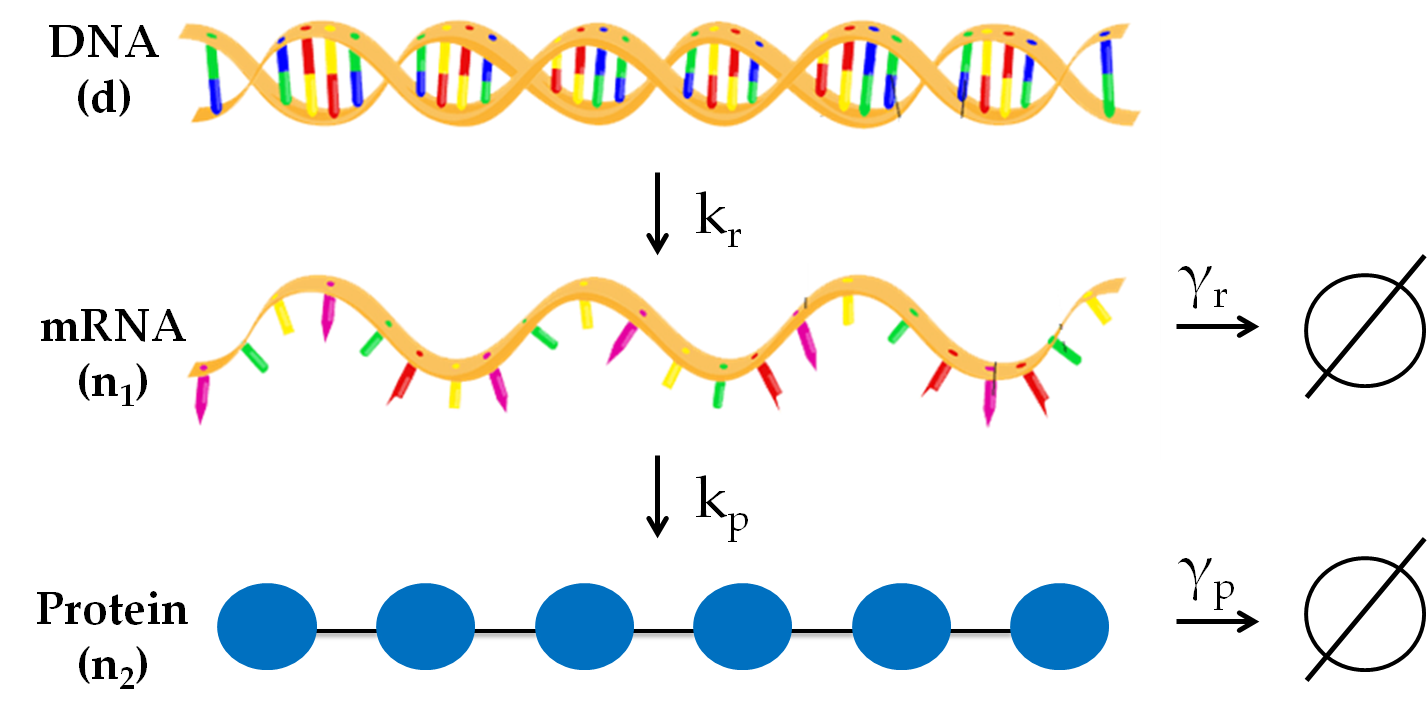
\includegraphics[width=8cm]{mas-dogma}
  \caption[Model of gene expression for a single gene]{\label{fig:mas-dogma} Steps of gene expression considered in the model. Taken from \cite{thattai01}.}
\end{figure}

According to the assumptions, the deterministic equations for $n_1$ and $n_2$ are

\begin{align}
  \dot{n_1}(t) &= k_rd-\gamma_rn_1(t)\label{eq:mas-simple_det_1},\\
  \dot{n_2}(t) &= k_pn_1(t)-\gamma_pn_2(t) \label{eq:mas-simple_det_2}.
\end{align}

Hence, on steady state

\todo[inline]{Explain steady state on concepts, what does it mean?}

\begin{align}
   n_{1,s} &= \frac{k_r}{\gamma_r} \label{eq:mas-simple_ss_1}, \\
   n_{2,s} &= \frac{k_p}{\gamma_p} n_{1,s} = \frac{k_pk_r}{\gamma_p\gamma_r} \label{eq:mas-simple_ss_2}.
\end{align}

Let $n_1(0) = n_2(0) = 0$. Then, the solutions of the differential equation for $n_1$ is

\begin{equation*}
  n_1(t) = n_{1,s}\left(1-e^{-\gamma_rt}\right).
\end{equation*}

Also, assuming $n_1$ is fixed at some value $n_1^*$, the solution for $n_2$ is similar

\begin{equation*}
  n_2(t) = n_{2,s}\left(1-e^{-\gamma_rt}\right),
\end{equation*}

with $n_{2,s}=\frac{k_p}{\gamma_p}n_1^*$. Figure \ref{fig:mas-detSol} shows a plot of the solution.

\begin{figure}[H]
  \centering
  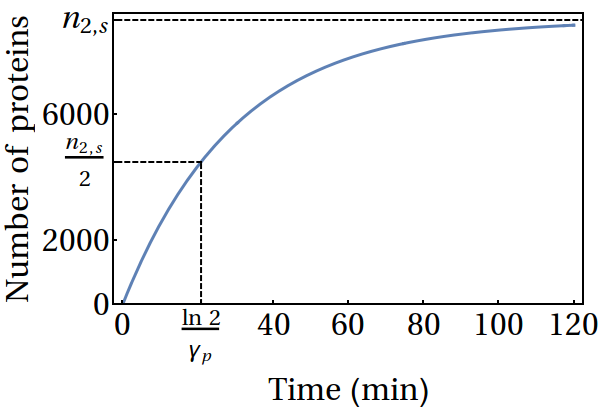
\includegraphics[width=13cm]{mas-detSol}
  \caption[Deterministic solution for the number of proteins]{\label{fig:mas-detSol} Deterministic solution for the number of proteins as a function of time for a fixed number of mRNAs. The time for reaching half the steady state value, $\ln 2/\gamma_p$, and the steady state value are marked with dashed lines.}
\end{figure}

The number of protein reaches half its steady state in a time of $\ln 2/\gamma_p$. Then, the speed at which $n_2$ reaches its steady state is proportional to $1/\gamma_p$ and it is the same independently of whether the levels start above or below $n_{2,s}$. If the number of mRNA molecules changes, the steady state level for $n_2$ also changes and the proteins reach the new steady state within a timescale of $1/\gamma_p$. This fact is very important in noise propagation as we will see in the next chapter.

A parameters that living beings might want to tune in their genetic circuits is their response time. In an unregulated gene $\gamma_p$ must be increased to have a faster response time. To do that, proteins must be actively destroyed and this raises the energetic cost. However, there are more sophisticated mechanisms to control the response time such as feed forward loops and autorregulation \cite{alon06}.

The solutions of the differential equations \eqref{eq:mas-simple_det_1} and \eqref{eq:mas-simple_det_2} are continous functions of time that are uniquely determined for some given initial conditions. However, in the reality $n_1$ and $n_2$ are discrete numbers. This fact determines an important part of their stochastic behaviour. Also, the synthesis and degradation of the molecules are, at a fundamental level, a consequence of random collisions of molecules that are difussing through the cell (e.g. mRNA polymerases with the promoter and enzymes with their substrates).

With this in mind, to account for the noise the quantities $n_1(t)$ and $n_2(t)$ are defined as stochastic processes instead of deterministic functions. Also, they only take values on $\mathbb{N}$ instead of $\mathbb{R}^+$. In the ME aproach, the system can be thought as a set of states labeled with all the possible pairs $(n_1,n_2)$. The rates of synthesis and degradation are thought as the probabilities per unit time of a transition between states occuring. Figure \ref{fig:mas-trans_single} shows the possible transitions from and into the state $(n_1,n_2)$.

\begin{figure}[H]
  \centering
  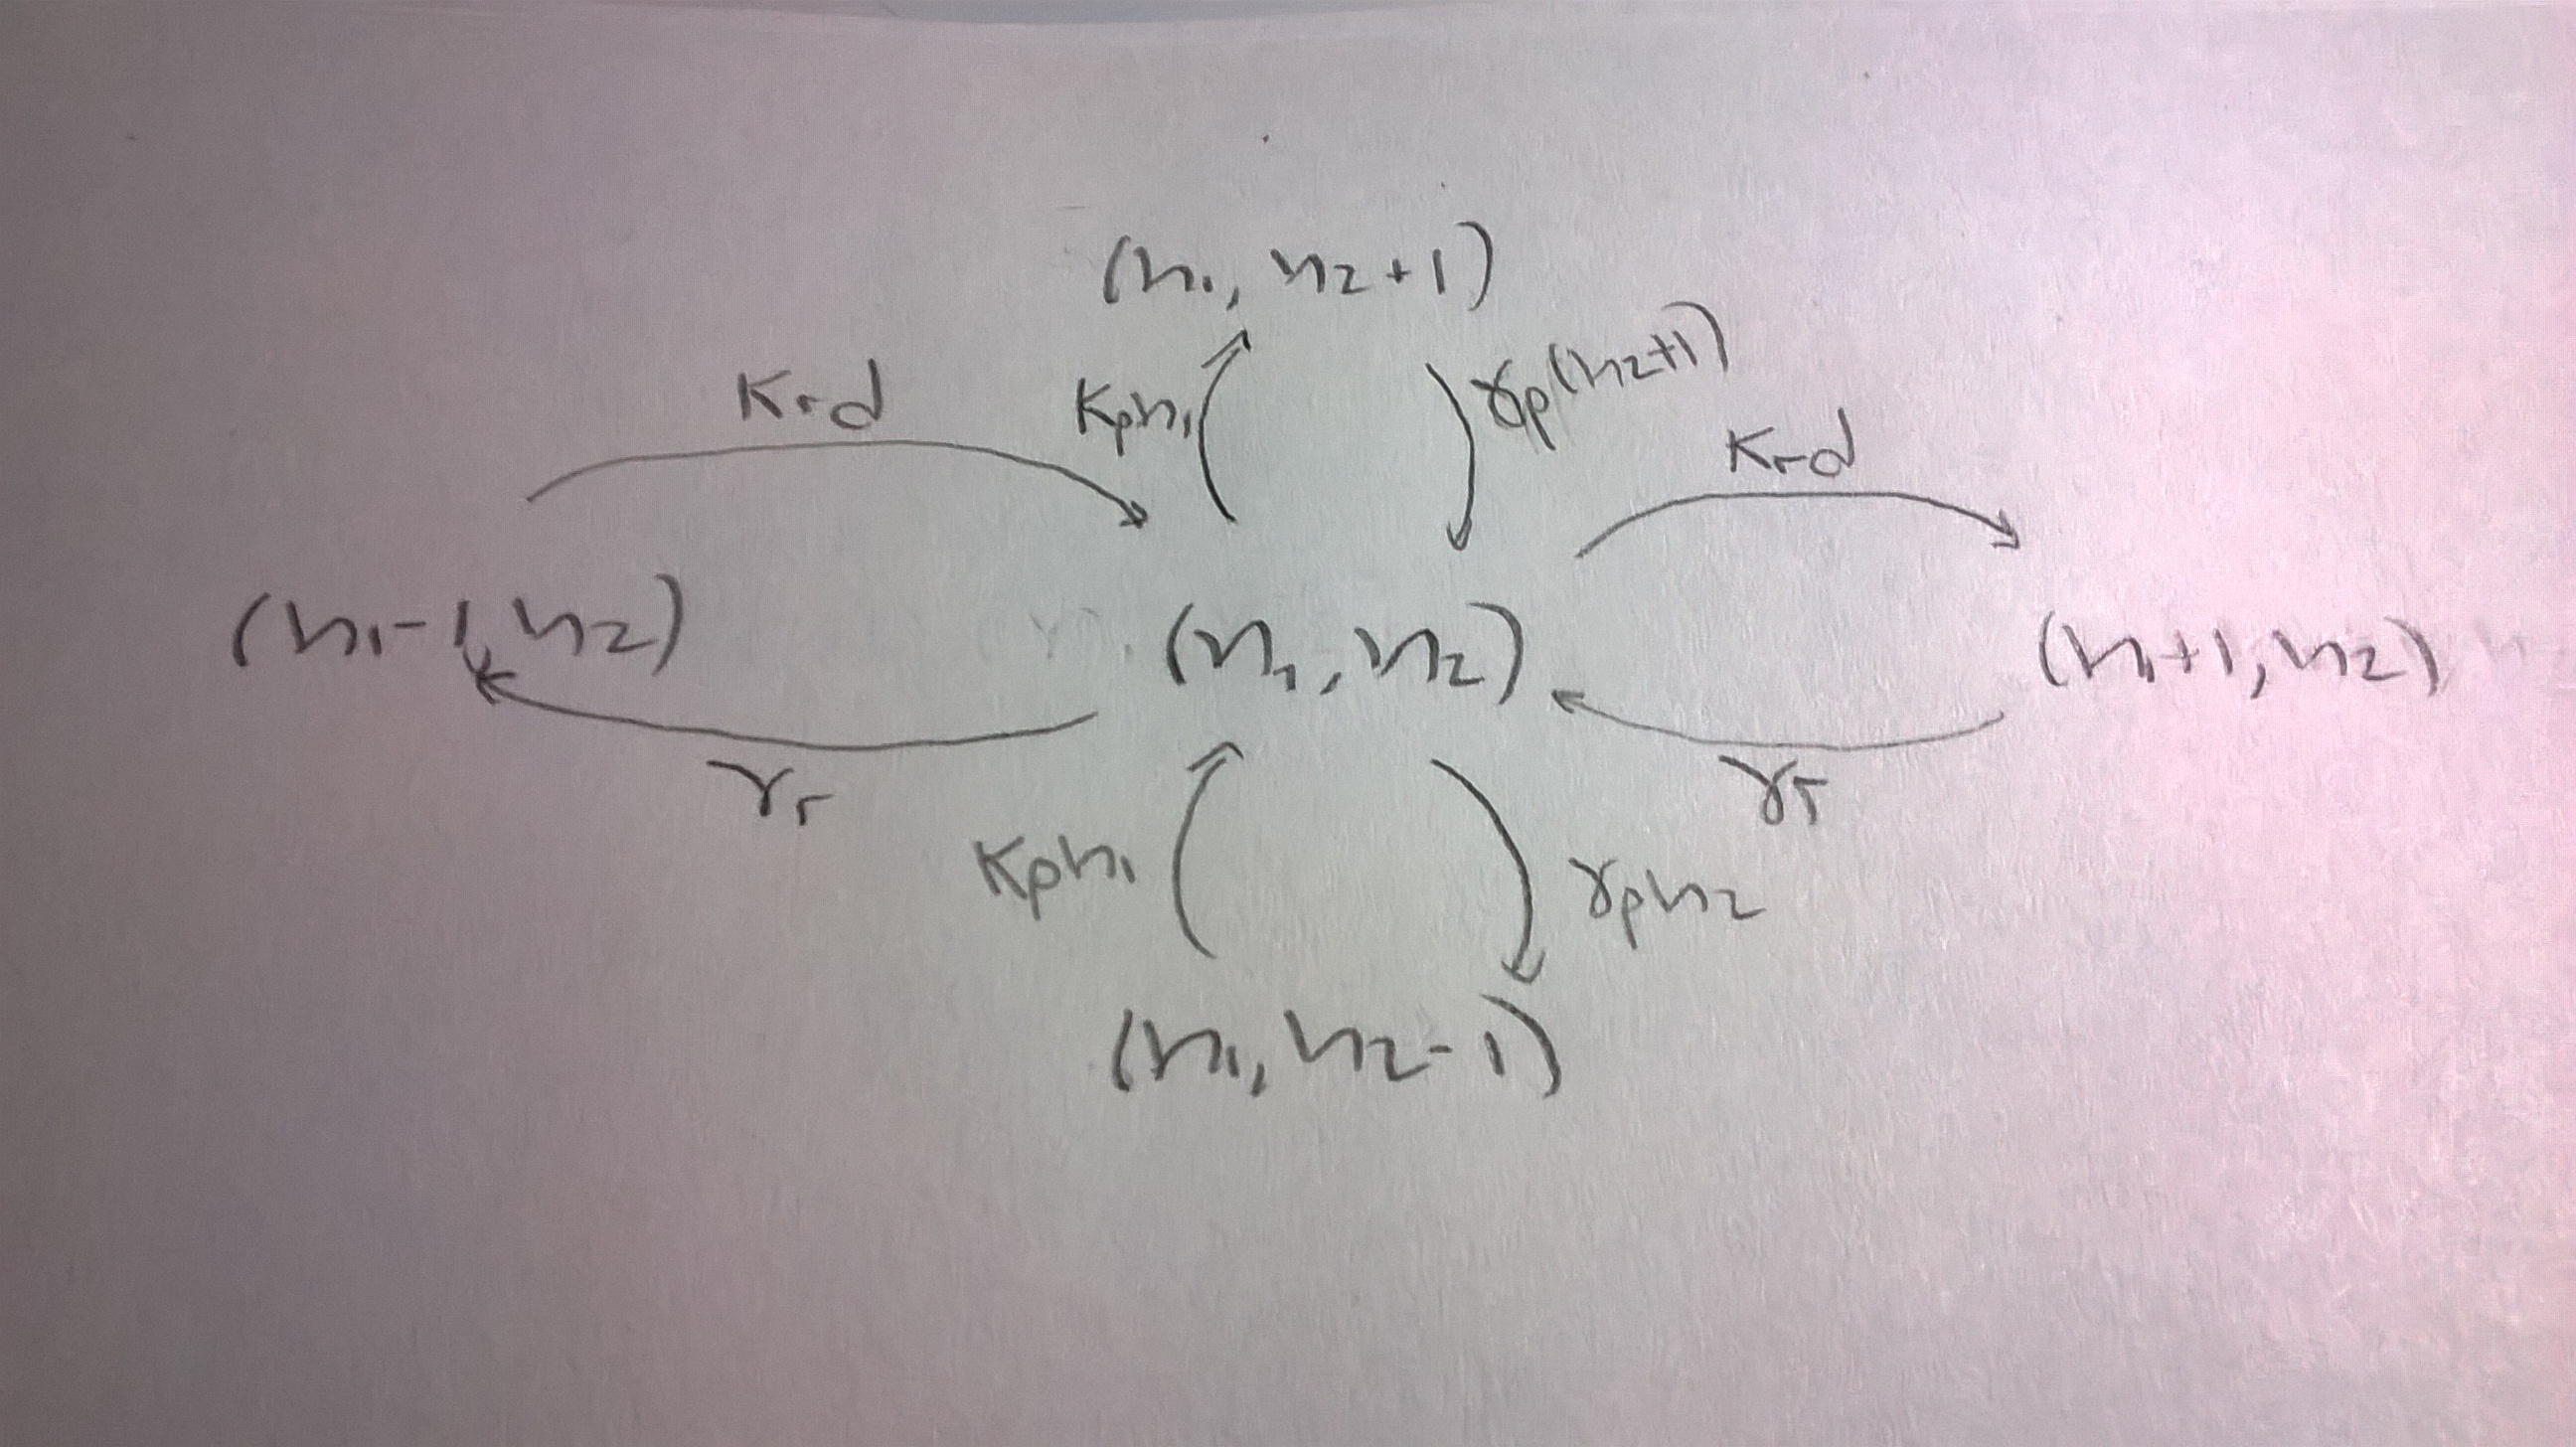
\includegraphics[width=8cm]{mas-trans_single}
  \caption[Transitions between states for a single gene]{\label{fig:mas-trans_single} Scheme of the possible transitions involving $n_1$ RNA molecules and $n_2$ protein molecules.}
\end{figure}

The transitions shown in figure \ref{fig:mas-trans_single} can be interpreted as follows: there is a probability $p(n_1,n_2,t)$ of being at the state $(n_1,n_2)$ at time $t$ which changes according to the probabilities of being in the adjacent states and the transition probabilities given by the reaction rates. Also, it is assumed that the probability of being at a state is independent of the transition probabilities. Formally speaking, applying the master equation approach implies that the processes are Markovian.

Therefore, to completely characterize the system under this scheme, the PMF $p(n_1,n_2,t)$ must be found for all possible $n_1$, $n_2$ and $t$. We can write a difference-differential equation for $p$ called the Master Equation, it is given by

\begin{equation}
  \label{eq:master}
  \begin{split}
    \frac{\mathrm{d}p(n_1,n_2,t)}{\mathrm{d}t} &= k_rdp(n_1-1,n_2,t) - k_rdp(n_1,n_2,t)\\
&+ k_pn_1p(n_1,n_2-1,t) - k_pn_1p(n_1,n_2,t)\\
&+ \gamma_r(n_1+1)p(n_1+1,n_2,t) - \gamma_rn_1p(n_1,n_2,t)\\
&+ \gamma_p(n_2+1)p(n_1,n_2+1,t) - \gamma_pn_2p(n_1,n_2+1,t).
  \end{split}
\end{equation}

The first term refers to a transition from state $(n_1-1,n_2,t)$ to $(n_1,n_2,t)$ via a creation of a mRNA molecule, whereas the second term involves a transition $(n_1,n_2,t) \rightarrow (n_1+1,n_2,t)$ via mRNA synthesis. The third and fourth terms have the meaning but related to protein synthesis. The other terms are related to transitions due to degradation.

\todo[inline]{Define moments}

The PMF can be found from the ME for certain systems. Nevertheless, to find the noise we only need the first and second moments. To do that we write the master equation in terms of the moment generating function $F(z_1,z_2)$, defined in eq. \eqref{def:mom_gen}. Multiplying by $z_1^{n_1}z_2^{n_2}$ and summing over $n_1$ and $n_2$, both from $0$ to $\infty$ we obtain for the left hand side simply $\dot{F}(z_1,z_2)$. For the first term on the right hand side we obtain \footnote{The time dependence is not shown for simplicity.}

\begin{equation*}
  \sum_{\mathclap{n_1=0,n_2=0}}^\infty z_1^{n_1}z_2^{n_2}f(n_1-1,n_2) = \sum_{\mathclap{n_1=-1,n_2=0}}^\infty z_1^{n_1+1}z_2^{n_2}f(n_1,n_2),
\end{equation*}

but since $n_1$ represents number of molecules, it must be a positive quantity. Hence $f(-1,n_2)=0$ and the last sum can be taken from $n_1=0$ yielding

\begin{equation*}
  z_1 \sum_{\mathclap{n_1=0,n_2=0}}^\infty z_1^{n_1}z_2^{n_2}f(n_1,n_2) = z_1F(z_1,z_2).
\end{equation*}

For the second term of eq. \eqref{eq:master} the result is trivial, for the third term we get

\begin{equation*}
  \sum_{\mathclap{n_1=0,n_2=0}}^\infty n_1f(n_1,n_2-1) = \sum_{\mathclap{n_1=0,n_2=-1}}^\infty n_1z_1^{n_1}z_2^{n_2+1}f(n_1,n_2).
\end{equation*}

Using the same argument as above, $f(n_1,-1) = 0$. Rearranging it becomes

\begin{equation*}
  z_1 z_2 \sum_{\mathclap{n_1=0,n_2=0}}^\infty z_1^{n_1-1}z_2^{n_2}f(n_1,n_2) = z_1 z_2 \frac{\partial F(z_1,z_2)}{\partial z_1}.
\end{equation*}

For the fifth term

\begin{equation*}
  \begin{split}
    \sum_{\mathclap{n_1=0,n_2=0}}^\infty (n_1+1)z_1^{n_1}z_2^{n_2}f(n_1+1,n_2) &= \sum_{\mathclap{n_1=1,n_2=0}}^\infty n_1z_1^{n_1-1}z_2^{n_2}f(n_1,n_2)\\ 
    &= z_1 \sum_{\mathclap{n_1=0,n_2=0}}^\infty n_1z_1^{n_1-1}z_2^{n_2}f(n_1,n_2) = \frac{\partial F(z_1,z_2)}{\partial z_1}.
  \end{split}
\end{equation*}

The other terms are treated in a similar fashion. Putting all of this together in we obtain the master equation in terms of the moment generating function $F$

\begin{equation}
  \label{eq:masterF}
  \begin{split}
    \dot{F}(z_1,z_2,t) &= k_rd(z_1-1)F(z_1,z_2,t) + k_pz_1(z_2-1)\frac{\partial F(z_1,z_2,t)}{\partial z_1} \\
    &+ \gamma_r(1-z_1)\frac{\partial F(z_1,z_2,t)}{\partial z_1} + \gamma_p(1-z_2)\frac{\partial F(z_1,z_2,t)}{\partial z_2}.
  \end{split}
\end{equation}

We transformed a difference equation in $(n_1,n_2)$ into a partial differential equation in $(z_1,z_2)$. The PMF $p$ can be found by solving for $F$ and transforming back. However, in this case we will use the properties of $F$ (eqs. \eqref{eq:con-mom_gen_1} - \eqref{eq:con-mom_gen_d1d1}) to find only the first two moments. Differentiating with respect to $z_1$

\begin{equation}
  \label{eq:dz1}
  \begin{split}
    \frac{\partial \dot{F}}{\partial z_1} &= k_rd\left( F+(z-1)\frac{\partial F}{\partial z_1} \right) + k_p(z_2-1) \left( \frac{\partial F}{\partial z_1} + z_1 \frac{\partial^2 F}{\partial z_1^2} \right)\\
    &+\gamma_r\left(-\frac{\partial F}{\partial z_1}+(1-z_1)\frac{\partial^2 F}{\partial z_1^2}\right)+\gamma_p(1-z_2)\frac{\partial^2 F}{\partial z_1 \partial z_2},
  \end{split}
\end{equation}

and with respect to $z_2$

\begin{equation}
  \label{eq:dz2}
  \begin{split}
    \frac{\partial \dot{F}}{\partial z_2}&=k_rd(z_1-1)\frac{\partial F}{\partial z_2} + k_pz_1\left(\frac{\partial F}{\partial z_1} + (z_2-1)\frac{\partial^2 F}{\partial z_1 \partial z_2} \right)\\
    &+ \gamma_r(1-z_1)\frac{\partial^2 F}{\partial z_1 \partial z_2} + \gamma_p\left(-\frac{\partial F}{\partial z_2}+(1-z_2)\frac{\partial^2 F}{\partial z_2^2}\right).
  \end{split}
\end{equation}

Evaluating eqs. \eqref{eq:dz1} and \eqref{eq:dz2} at $z_1 = z_2 = 1$ and using properties \eqref{eq:con-mom_gen_1} and \eqref{eq:con-mom_gen_d1} we obtain

\begin{align*}
\dot{\langle n_1 \rangle}&= k_rd - \gamma_r \langle n_1 \rangle,\\
\dot{\langle n_2 \rangle}&= k_p\langle n_1 \rangle - \gamma_p \langle n_2 \rangle.
\end{align*}

Which are the same as eqs. \eqref{eq:mas-simple_det_1} and \eqref{eq:mas-simple_det_2}. Therefore, the averages follow the deterministic behavior and the steady state values are thus given by eqs. \eqref{eq:mas-simple_ss_1} and \eqref{eq:mas-simple_ss_2}. 

Differentiating eq. \eqref{eq:dz1} with respect to $z_2$, eq. \eqref{eq:dz1} with respect to $z_1$ and eq. \eqref{eq:dz2} with respect to $z_2$ and evaluating at $z_1 = z_2 = 1$ we obtain, respectively

\begin{align}
  \dot{\langle n_1n_2\rangle} &= k_rd\langle n_2 \rangle + k_p\left(\langle n_1\rangle + \langle n_1(n_1-1) \rangle \right) - \left( \gamma_r + \gamma_p \right)\langle n_1n_2 \rangle,\label{eq:dz1z2}\\
  \dot{\langle n_1(n_1-1)\rangle} &= 2k_r\langle n_1\rangle-2\gamma_r\langle n_1(n_1-1) \rangle, \label{eq:dz1z1}\\
  \dot{\langle n_2(n_2-1)\rangle} &= 2k_p\langle n_1n_2 \rangle - 2\gamma_p\langle n_2(n_2-1)\rangle. \label{eq:dz2z2}
\end{align}

The previous equations will be treated in steady state. From  eq. \eqref{eq:dz1z1}

\begin{equation}
  \label{eq:pren1}
  0 = k_rd \langle n_1 \rangle_s -\gamma_r \left(\langle n_1^2 \rangle_s - \langle n_1 \rangle_s \right) \Rightarrow \langle n_1^2 \rangle_s = \frac{k_rd}{\gamma_r}\langle n_1 \rangle_s + \langle n_1 \rangle_s = \langle n_1 \rangle_s^2 + \langle n_1 \rangle_s.
\end{equation}

Therefore, in steady state $\sigma_1^2 = \langle n_1 \rangle$. Hence, the Fano factor and the squared CV for the mRNA are given by

\begin{equation}
  \label{noise1}
  \nu_1 = 1, \quad\quad \eta_1^2 = \frac{1}{\langle n_1 \rangle}.
\end{equation}

Which is the noise for a Poisson process as we saw on eq. \eqref{eq:con-poisson_noise}. This makes sense since the assumptions made for the mRNA dynamics correspond to the ones made for the Poisson process in section \ref{sec:poisson}. In \textit{E. coli}, $\langle n_1\rangle_s ~ 5$ mRNA molecules. Since the number is low, the mRNA number present large fluctuations.

From eq. \eqref{eq:dz1z2} we have

\begin{equation*}
  0 = k_rd \langle n_2 \rangle_s + k_p \langle n_1^2 \rangle_s - (\gamma_p + \gamma_r) \langle n_1n_2 \rangle_s \Rightarrow \langle n_1n_2 \rangle_s  = \frac{k_rd\langle n_2\rangle_s+k_p\langle n_1^2\rangle_s}{\gamma_r+\gamma_p}.
\end{equation*}

But from eq. \eqref{eq:pren1} and \eqref{eq:mas-simple_ss_2},

\begin{equation}
\langle n_1^2 \rangle_s = \langle n_1 \rangle_s\left( \langle n_1 \rangle_s+1\right) = \frac{\gamma_p}{k_p}\langle n_2 \rangle_s\left(\langle n_1\rangle_s + 1\right).
\end{equation}

Hence, the covariance is given by

\begin{align*}
  \langle n_1n_2 \rangle_s - \langle n_1 \rangle_s\langle n_2\rangle_s &= \langle n_2 \rangle_s \left(\frac{k_rd+\gamma_p\left(\langle n_1\rangle_s+1\right)}{\gamma_r+\gamma_p}-\langle n_1\rangle_s\right)\\
  &=\langle n_2\rangle_s\frac{k_rd+\gamma_p-\gamma_r\langle n_1\rangle_s}{\gamma_r+\gamma_p}.
\end{align*}

From eq. \eqref{eq:mas-simple_ss_1} the first and third term of the numerator cancel out, therefore

\begin{equation}
  \label{eq:cov12}
  \boxed{\text{cov}(n_1,n_2)_s = \langle n_2 \rangle_s\frac{\frac{\gamma_p}{\gamma_r}}{1+\frac{\gamma_p}{\gamma_r}}}.
\end{equation}

From eq. \ref{eq:dz2z2} we have

\begin{equation*}
kp\langle n_1n_2\rangle_s = \gamma_p\langle n_2^2\rangle_s-\gamma_p\langle n_2\rangle_s
\end{equation*}

Replacing eq. \ref{eq:cov12} in the previous equation we get after rearranging

\begin{align*}
  \langle n_2^2\rangle_s &= \frac{k_p}{\gamma_p}\left(\langle n_1 \rangle_s\langle n_2\rangle_s + \frac{\langle n_2\rangle_s\gamma_p}{\gamma_r+\gamma_p}\right) + \langle n_2 \rangle_s\\
  &=\langle n_2^2\rangle_s+\frac{k_p\langle n_2\rangle_s}{\gamma_r+\gamma_p}+\langle n_2 \rangle_s.
\end{align*}

Hence substracting $\langle n_2\rangle_s^2$ from the previous equation we obtain

\begin{equation*}
  \sigma_2^2 = \langle n_2\rangle\left(\frac{\nicefrac{k_p}{\gamma_r}}{1+\nicefrac{\gamma_p}{\gamma_r}}+1\right).
\end{equation*}

Therefore, the noise for the proteins in steady state is given by

\begin{equation}
  \label{eq:noise2}
  \nu_2 = \frac{b}{1+\nicefrac{\gamma_p}{\gamma_r}}+1, \quad \quad \eta_2^2 = \frac{1}{\langle n_2\rangle}\left(\frac{b}{1+\nicefrac{\gamma_p}{\gamma_r}}+1\right).
\end{equation}

\todo[inline]{Explain something about orders of magnitude}

where $b\coloneqq k_p/\gamma_r$ is the average number of proteins that are produced during the lifetime of a transcript, often called the \textit{burst size}. The second part ($1$ in $\nu_p$) is the Poisson noise, which measured as the CV is negligible because the average number of proteins for a given gene is usually large (of the order of $1000$ to $10000$ in \textit{E. coli}).

The first part is the contribution to the noise that arises in mRNA fluctuations and is propagated to the proteins since they are related by the rate of production of proteins $k_pn_1$. The noise in the number of proteins is thus much larger than Poissonian since $b$ is about $15$ proteins/mRNA. The factor $1/(1+\gamma_p/\gamma_r)$ represent the so called time averaging of fluctuations, it takes values between $0$ and $1$. Usually $\gamma_p<\gamma_r$, meaning that fluctuations in mRNA number happen on a characteristic timescale $\tau_r \propto 1/\gamma_r$  that is smaller than the response time of the proteins $\tau_p \propto 1/\gamma_p$. The proteins are thus unable to respond immediately to the mRNA fluctuations. As a consequence, the protein make a time average over many ups and downs of mRNA. This process reduces fluctuations in the number of proteins. This very important phenomenon will be considered with more detain in section \ref{sec:fdt-time-ave}.

The analytical results are compared with the results of Gillespie simulations in fig. \ref{fig:mas-sim_simple}. It can be seen that the Fano factor is strongly dependent on the burst size $b$, independent of $k_r$ and dependent on the protein half-life $\tau_p = \ln2/\gamma_r$ only for low values of $\langle p\rangle$. Also, $\nu_p$ can become much larger than $1$ for biologically relevant parameters, verifying that the noise of proteins is much larger than Poisson.

\begin{figure}[H]
  \centering
  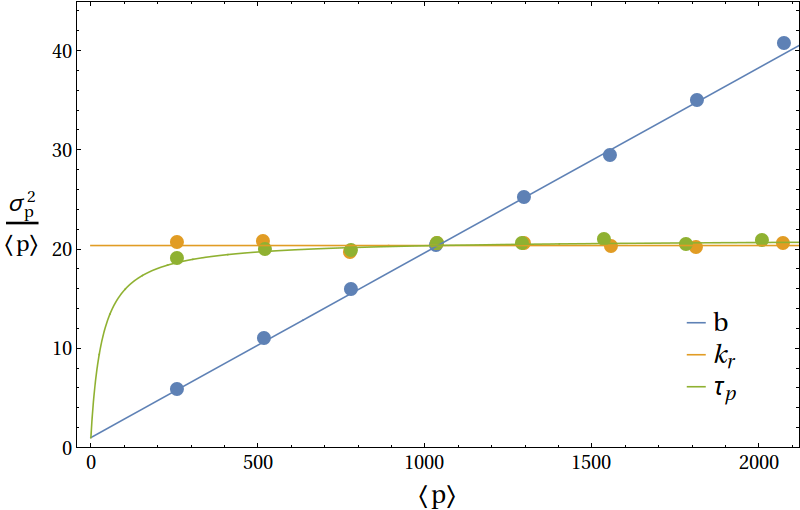
\includegraphics[width=13cm]{mas-sim_simple}
  \caption[Noise in proteins: comparing analytical results and Gillespie simulations]{\label{fig:mas-sim_simple} Comparison between the results of Gillespie simulations (dots) and the analytical results (lines) given by eq. \eqref{eq:noise2}. The Fano factor is plotted vs. the mean number of proteins in steady state. The base values of the parameters are $\tau_r = \ln2/\gamma_r = 2$ min,  $b=20$ proteins/mRNA $k_r = 0.01$ mRNA/s and $\tau_p = \ln2/\gamma_p = 1$ h. For each curve, the parameter indicated in the legend is varied while the others are fixed. $b$ is varied between $5$ and $40$ proteins/mRNA; $k_r$ varies between $0.0025$ and $0.02$ mRNA/s; and $\tau_p$ varies from $15$ min to $2$ h. Each point correspond to $10000$ trials where each one was evolved until a time of $10\tau_p$ in order to be sure that the system has reached its steady state \footnotemark.}
\end{figure}

\todo[inline]{Define the thing with kr and krd}

\footnotetext{The simulations were programmed in C and the graphics were done with Wolfram Mathematica. The scripts can be found \href{https://github.com/gutiloluis/61Monograph/tree/master/mas-gillespie}{here}.} 

The noise and the steady state average in protein numbers can be controlled independently by controlling the burst size $b$. If a cell produces many mRNAs and a few proteins per transcript (small $b$), the noise is reduced. On the contrary, the same average number of proteins can be reached by producing a few mRNAs and many proteins per mRNA (large $b$). In this case the noise is larger. Nevertheless, reducing noise in this case requires a constant synthesis and degradation of many mRNAs. This is inefficient for the cells since they are spending energy in the production of mRNAs from which there will be only a few proteins translated. This suggests that there is an interchange between fitness and noise reduction in the cells that has been tuned by evolution according to the necessity of reliability of the particular genetic component. However, we will see that there are other mechanisms, like negative autorregulation (sec. \ref{sec:mas-neg_autorreg}), that allow cells to reduce noise in a more efficient way.

\todo[inline]{Define fitness, word for pay-off}

\section{Several species with linear interactions}

In this section we generalize the previous results to arbitrary genetic network in which the interactions between its components are linear. Consider eqs. \eqref{eq:mas-simple_det_1} and \eqref{eq:mas-simple_det_2}. In matrix notation, they can be written as

\begin{equation}
  \label{eq:matdet}
  \mathbf{\dot{n}} = \left( \mathbf{A} - \mathbf{\Gamma} \right) \mathbf{n},
\end{equation}

where $\mathbf{n}^T=(d,n_1,n_2)$ is the vector of chemical species and the matrices $\mathbf{A}$ and $\mathbf{\Gamma}$ are defined as

\todo[inline]{Try to write eqs. on the same line}

\begin{align}
  \mathbf{A} &=
  \begin{pmatrix}
    0 & 0 & 0 \\
    k_r & 0 & 0 \\
    0 & k_p & 0
  \end{pmatrix} \label{eq:mas_A_single},\\
  \mathbf{\Gamma} &=
  \begin{pmatrix}
    0 & 0 & 0 \\
    0 & \gamma_r & 0 \\
    0 & 0 & \gamma_p 
  \end{pmatrix} \label{eq:mas_G_single}. 
\end{align}

$\mathbf{A}$ contains the creation rates and describes how each rate depends on the different species and $\mathbf{\Gamma}$ has the degradation rates, which is diagonal whenever the degradation is not mediated by interactions among different kinds of molecules.

For an arbitrary circuit with an arbitrary number $N$ of species and linear interaction between them, we can write its deterministic equations in the form of eq. \eqref{eq:matdet}. In the ME approach for genetic circuits, the state space has now $N$ dimensions and the ME has now $4N$ terms. This is because for each kind of molecule there are two transitions given by synthesis and two given by degradation as can be seen in fig. \ref{fig:mas-trans_single}. With this in mind, the ME is given by \footnote{To reduce the complexity of the expressions, we define $p(n_i) \coloneqq p(\mathbf{n}) = p(n_1,\dotsc,n_i,\dotsc,n_N)$, and $p(n_i\pm1)\coloneqq p(n_1,\dotsc,n_i\pm1,\dotsc,n_N)$. The same convention is used for $F(z_i)$.}

\begin{equation}
  \label{eq:masterg1}
  \dot{p}(n_i) =  \sum_{i=1}^N\left(\sum_{j=1}^N A_{ij}n_j \left( p(n_i-1) - p(n_i) \right) + \sum_{j=1}^N \Gamma_{ij}((n_j+1)p(n_i+1)-n_jp(n_i))\right)
\end{equation}

When for a fixed specie $i$, the terms in parentheses represent having $n_i-1$ molecules of the $i$th type and creating one; having $n_i$ and creating one; having $n_i+1$ and destroying one; and having $n_i$ and destroying one, respectively. Since this is possible for each of the $N$ types of molecules, we must sum over $i$ as well.

Assuming that degradation does not involve interactions between various molecules, the matrix $\Gamma$ can be taken to be diagonal, i.e. $\Gamma_{ij}=\delta_{ij}\Gamma_j$. With this eq. \eqref{eq:masterg1} becomes

\begin{equation}
\label{eq:masterg2}
\dot{p}(n_i) =  \sum_{i=1}^N\left(\sum_{j=1}^N A_{ij}n_j \left( p(n_i-1) - p(n_i) \right) + \Gamma_{i}((n_i+1)p(n_i+1)-n_ip(n_i))\right).
\end{equation}

To find the mean and variances, we write the master equation in terms of the moment generating function and use its properties to find equations for the moments. In this case we multiply by $z_1^{n_1}\dotsm z_N^{n_N}$ and sum over $n_1,\dotsc n_N$, all from $0$ to $\infty$. First we will consider the term in parentheses of eq. \eqref{eq:masterg2} and later we will perform the outer sum over $i$. For the first term we obtain the following expression \footnote{To avoid unnecesarily long expressions, we write $\sum$ refering to $\sum_{n_1=0}^\infty\dotsi\sum_{n_N=0}^\infty$.}

\begin{equation}
  \label{eq:momg1}
  \sum n_j z_1^{n_1}\dotsm z_i^{n_i}\dotsm z_j^{n_j}\dotsm z_N^{n_N} f(n_i) = z_iz_j\sum n_jz_j^{n_j-1}z_i^{n_i}f(n_i) = z_iz_j\frac{\partial F}{\partial z_j}. 
\end{equation} 

Where the index switching trick used previously was used. Similarly, for the second term

\begin{equation}
  \label{eq:momg2}
  \sum n_jz_j^{n_j}z_i^{n_i}f(n_i) = z_j\frac{\partial F}{\partial z_j}.
\end{equation}

For the third and fourth terms

\begin{equation}
  \label{eq:momg3}
  \sum (n_i+1)z_i^{n_i}f(n_i+1) = \sum n_i z_i^{n_i-1}f(n_i) = \frac{\partial F}{\partial z_i},
\end{equation}

\begin{equation}
  \label{eq:momg4}
  \sum n_iz_i^{n_i}f(n_i) = z_i\frac{\partial F}{\partial z_i}.
\end{equation}

Replacing eqs. \eqref{eq:momg1} - \eqref{eq:momg4} in eq. \eqref{eq:masterg2} yields the equation for the moment generating function

\begin{equation}
\dot{F}(z_i) = \sum_i\left( z_i\sum_jA_{ij}\frac{\partial F}{\partial z_j} - \sum_jA_{ij} z_j \frac{\partial F}{\partial z_j} + \Gamma_i\frac{\partial F}{\partial z_i} - \Gamma_iz_i\frac{\partial F}{\partial z_i}\right),
\end{equation}

which after factoring becomes

\begin{equation}
\label{eq:momg}
\dot{F}(z_i) = \sum_i(z_i-1)\left(\sum_jA_{ij} z_j \frac{\partial F}{\partial z_j} - \Gamma_i\frac{\partial F}{\partial z_i}\right).
\end{equation}

We have to differentiate it and use the properties \eqref{eq:con-mom_gen_d1} - \eqref{eq:con-mom_gen_d1d1} to obtain equations for the moments. Differentiating with respect to $z_l$

\begin{equation*}
\begin{split}
\frac{\partial \dot{F}}{\partial z_l} &= \sum_i\left[(z_i-1)\left[\sum_jA_{ij}\left(\delta_{jl}\frac{\partial F}{\partial z_j}+z_j\frac{\partial^2 F}{\partial z_j\partial z_l}\right)-\Gamma_i\frac{\partial^2 F}{\partial z_i\partial z_l}\right]\right.\\
&+\left.\delta_{il}\left(\sum_jA_{ij}z_j\frac{\partial F}{\partial z_j}-\Gamma_i\frac{\partial F}{\partial z_i}\right)\right].
\end{split}
\end{equation*}

\begin{equation*}
\begin{split}
\frac{\partial \dot{F}}{\partial z_l} &= \sum_i(z_i-1)\left[A_{il}\frac{\partial F}{\partial z_l}+\sum_jA_{ij}z_j\frac{\partial^2 F}{\partial z_j\partial z_l}-\Gamma_i\frac{\partial^2 F}{\partial z_i\partial z_l}\right]\\
&+\sum_jA_{lj}z_j\frac{\partial F}{\partial z_j}-\Gamma_l\frac{\partial F}{\partial z_l}.
\end{split}
\end{equation*}

Evaluating in $z_i=1$, $i=1,\dotsc,N$ we otain after applying the properties of $F$

\begin{equation*}
\dot{\langle n_l \rangle} = \sum_jA_{lj}\langle n_j\rangle-\Gamma_l\langle n_l\rangle,
\end{equation*}

and writing in matrix form

\begin{equation}
  \label{eq:mas-general_ave}
  \dot{\langle \mathbf{n}\rangle} = (\mathbf{A}-\mathbf{\Gamma})\langle \mathbf{n}\rangle,
\end{equation}

as expected. It has the same form of the deterministic equations \eqref{eq:matdet}. Differentiating again with respect to $z_m$ and doing some algebra

\begin{equation*}
  \begin{split}
    \frac{\partial^2 \dot{F}}{\partial z_l \partial z_m} &= \sum_i(z_i-1) \left(A_{im}\frac{\partial^2F}{\partial z_i \partial z_m} + \sum_jA_{ij}z_j\frac{\partial^3F}{\partial z_j \partial z_l \partial z_m}+A_{il}\frac{\partial^2F}{\partial z_l\partial z_m} - \Gamma_i\frac{\partial^3F}{\partial z_i \partial z_l \partial z_m}   \right)\\
    &+\sum_jA_{mj}z_j\frac{\partial^2F}{\partial z_j\partial z_l}+A_{ml}\frac{\partial F}{\partial z_l} - \Gamma_m\frac{\partial^2F}{\partial z_l\partial z_m}\\
    &+ A_{lm}\frac{\partial F}{\partial z_m} + \sum_jA_{lj}z_j\frac{\partial^2F}{\partial z_j\partial z_m}-\Gamma_l\frac{\partial^2F}{\partial z_l\partial z_m}.
  \end{split}
\end{equation*}

Evaluating at $z_i=1$ for all $i$

\begin{equation*}
  \frac{\partial^2\dot{F}}{\partial z_l \partial z_m} = \sum_jA_{mj}z_j\frac{\partial^2F}{\partial z_j\partial z_l}+A_{ml}\frac{\partial F}{\partial z_l} - \Gamma_m\frac{\partial^2F}{\partial z_l\partial z_m} + A_{lm}\frac{\partial F}{\partial z_m} + \sum_jA_{lj}z_j\frac{\partial^2F}{\partial z_j\partial z_m}-\Gamma_l\frac{\partial^2F}{\partial z_l\partial z_m}.
\end{equation*}

Rearranging the previous eq. and using again the fact that $\mathbf{\Gamma}$ is diagonal

\begin{equation*}
  \begin{split}
    \frac{\partial^2\dot{F}}{\partial z_l \partial z_m} &= \sum_j\left(A_{mj}z_j-\Gamma_{mj}\right)\frac{\partial^2F}{\partial z_j\partial z_l} + \sum_jA_{mj}\delta_{jl}\frac{\partial F}{\partial z_j}\\
    &+\sum_j\left(A_{lj}z_j-\Gamma_{lj}\right)\frac{\partial^2F}{\partial z_j\partial z_m} + \sum_jA_{lj}\delta_{jm}\frac{\partial F}{\partial z_j},
  \end{split}
\end{equation*}

This is valid for all $l$ and $m$. Evaluating at $z_i=1$ for all $i$ we get in matrix form

\begin{equation}
  \label{eq:mas-general}
  \nabla\nabla^T\dot{F}|_1 = \left(\left(\mathbf{\Gamma} - \mathbf{A}\right)\nabla\nabla^TF|_1 - \mathbf{A}\mathbf{\Theta} F|_1\right)+\left(\left(\mathbf{\Gamma} - \mathbf{A}\right)\nabla\nabla^TF|_1 - \mathbf{A}\mathbf{\Theta} F|_1\right)^T,
\end{equation}

where $\Theta_{ij} \coloneqq \delta_{ij}\frac{\partial}{\partial z_i}$. The set of linear equations can be solved for the moments and correlation using a computer program. Given the specific form of the matrices $\mathbf{A}$ and $\mathbf{\Gamma}$, we only have to replace on eq. \eqref{eq:mas-general_ave} and \eqref{eq:mas-general} to find the moments and the noise.

\section{Application to non-linear interactions: negative autorregulation}
\label{sec:mas-neg_autorreg}

As we have seen on sec. \ref{sec:hill}, the interactions between the component of a genetic circuits are non-linear. A consequence of this is that there might be several steady states. To apply the developed linear approach to such kind of systems we need to identify the stable fixed points, linearize about each of them, each linearization yields to a pair of matrices $\mathbf{A}$ and $\mathbf{\Gamma}$  that are replaced on eqs. \eqref{eq:mas-general_ave} and \eqref{eq:mas-general} to find the noise.

We will consider the case of negative autorregulation, in this case $k_r$ is now a Hill function for a repressor (eq. \eqref{eq:con-hillac}) that depends on the number of proteins of the same gene. Assuming that the basal transcription rate is $0$, the deterministic equations are

\begin{equation}
  \label{eq:mas-autorr_det}
  \begin{split}
    \dot{n_1}(t) &= k_r(n_2)d - \gamma_rn_1(t),\\
    \dot{n_2}(t) &= k_pn_1(t)-\gamma_pn_2(t),
  \end{split}
\end{equation}

where

\begin{equation*}
  k_r(n_2) \coloneqq \frac{k_r^{\text{max}}}{1+\left(\frac{n_2(t)}{K_d}\right)^n}.
\end{equation*}

Since the protein represses the transcription of his own gene, it is expected that the steady state number of proteins $\langle n_2\rangle_s$ is reduced with respect to the unrepressed case. To evidence this, fig. \ref{fig:mas-sim_hist} shows the distributions at steady state for the number of proteins of an unregulated and a negatively autorregulated gene resulting from Gillespie simulations. Both the average and the noise (width of the distribution) is reduced. The reduction of the noise occurs because a fluctuation that, for instance, increases the number of protein above the steady state level also increases the repression. This lowers the production rate, thus driving the levels back to the steady state with more strenght than in the unrepressed case. The effect is analogous for a random decrease of the level of proteins below steady state.

\todo[inline]{See if noise is actually reduced (reducing the width)}

\begin{figure}[H]
  \centering
  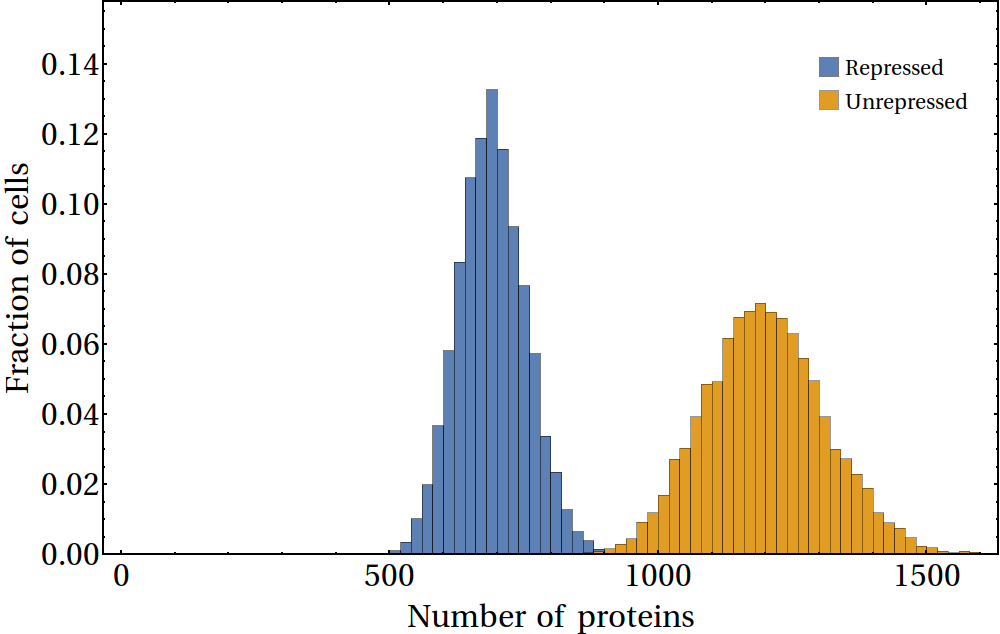
\includegraphics[width=13cm]{mas-hist}
  \caption[Histograms for protein number for a constitutive gene and a negatively autorregulated gene]{\label{fig:mas-sim_hist}Distribution for the number of proteins for an autorrepressed gene (eq. \ref{eq:mas-autorr_det}, blue), and an unrepressed gene (eqs. \ref{eq:mas-simple_det_1} and \ref{eq:mas-simple_det_2} with $k_r = k_r^\text{max}$, orange). The  values of the parameters are $\tau_r=2$ min, $\tau_p=1$ h, $b=10$ proteins/mRNA, $n=2$, $K_d=800$ proteins, and the average number of proteins without repression $\langle p\rangle_\text{unrep} \coloneqq k_r^\text{max}k_p/(\gamma_r\gamma_p) = 1200$ proteins. A sample of $10000$ cells (trials) evolved until a time of $10\tau_p$ was run on each histogram.}
\end{figure}

Next we find the average and Fano factor of $n_2$ according to the linearized model. Making a first order Taylor expansion of $k_r(n_2)$ about its value at the steady state $k_r(\langle n_2\rangle_s)$

\begin{equation}
  \begin{split}
  k_r(n_2) &\approx k_r(\langle n_2\rangle_s) + \left.\frac{\mathrm{d}k_r(n_2)}{\mathrm{d}n_2}\right|_{\langle n_2\rangle_s}\left(n_2-\langle n_2\rangle_s\right)\\
  &=\frac{k_r^{\text{max}}}{1+\left(\frac{\langle n_2\rangle_s}{K_d}\right)^n} - \frac{k_r^{\text{max}}n\left(\frac{\langle n_2\rangle_s}{K_d}\right)^{n-1}}{K_d\left(1+\left(\frac{\langle n_2\rangle_s}{K_d}\right)^n\right)^2}\left(n_2-\langle n_2\rangle_s\right)\\
  &= k_0-\frac{k_1}{d}n_2,
  \end{split}
\end{equation} 

where $k_0$ and $k_1$ are given by

\begin{equation*}
  k_0\coloneqq k_r(\langle n_2\rangle_s) - \left.\frac{\mathrm{d}k_r(n_2)}{\mathrm{d}n_2}\right|_{\langle n_2\rangle_s}\langle n_2\rangle_s,\quad\quad k_1 \coloneqq -\left.\frac{\mathrm{d}k_r(n_2)}{\mathrm{d}n_2}\right|_{\langle n_2\rangle_s}n_2. 
\end{equation*}

Therefore, the matrix $\mathbf{A}$ becomes

\begin{equation*}
  \mathbf{A} =
  \begin{pmatrix}
    0 & 0 & 0 \\
    k_0 & 0 & -k_1 \\
    0 & k_p & 0
  \end{pmatrix}
\end{equation*}

and $\mathbf{\Gamma}$ is the same as in \eqref{eq:mas_G_single}. Solving eqs. \eqref{eq:mas-general_ave} and \eqref{eq:mas-general} we get for the proteins in steady state

\begin{equation}
  \label{eq:mas-autorreg_final}
  \boxed{\langle n_2\rangle = \frac{1}{1+b\phi}\frac{k_0b}{\gamma_p}},\quad\quad \boxed{\nu_2 = \frac{1-\phi}{1+b\phi}\frac{b}{1+\frac{\gamma_p}{\gamma_r}}+1},
\end{equation}

with $\phi\coloneqq k_1/\gamma_p$ represents the strength of the feedback. In figure \ref{fig:mas-sim_autorreg}, we compare eq. \eqref{eq:mas-autorreg_final}  with a Gillespie simulation using the exact rates. Altought the analytic expressions are approximate, there is an excellent match with the simulations.

\begin{figure}[H]
  \centering
  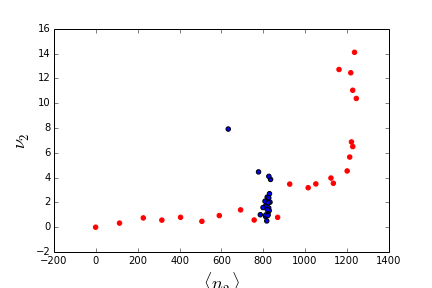
\includegraphics[width=13cm]{mas-sim_autorreg}
  \caption[Fano factor of protein number for a negatively autorregulated gene]{\label{fig:mas-sim_autorreg} Comparison between the results of Gillespie simulations (dots) using the exact eqs. \eqref{eq:mas-autorr_det} and the analytical results given by eq. \eqref{eq:mas-autorreg_final}. The Fano factor is plotted vs. the mean number of proteins in steady state. The base values of the parameters are the same as in fig. \ref{fig:mas-sim_hist}. For each curve, the parameter indicated in the legend is varied while the others are fixed. $K_d$ is varied from $100$ to $2000$ in increments of $100$ and from $2000$ to $5000$ in increments of $1000$, while $n$ is varied from $0$ to $20$ in unit increments. Each point correspond to 10000 trials. Each one evolved until a time of $10\tau_p$.}
\end{figure}

For a given average number of proteins, this circuit has a more efficient control of fluctuations than the one for the unrepressed gene. In this case, the random fluctuations are controlled by the same number of proteins and there is no need to spend energy in unused mRNA molecules. Evolution might have developed circuits of this kind, and more sophisticated, to tune the noise according to the function of the circuits trying to reduce the cost in fitness.

\section{Limitations of the model}

The linearized model has reliably reproduced the noise in steady state of two simple genetic circuits. We have also seen that it allows to consider an arbitrary number of species, allowing then to treat networks of arbitrary complexity. However, the model have some limitations. If the system is nonlinear, The nonlinearities should be such that the linearization correctly reproduces the behavior near the fixed points i.e. the nonlinearities should not be too large. Besides, this approach does not work for oscillating systems or unstable steady state points because in both mechanisms there may be large sudden changes in the average values that are not reproducible with a linear model.

However, phenomena such that big nonlinearities and oscillations is common in biological circuits and has allowed living beings to have many complex and interesting behaviors. Those features can not be studied with this model. Also, for many systems it would be important to model the complete time dynamics of noise, not just the steady state values. For example, the stochastic switching between different steady state values. 

\todo[inline]{Define fixed points, write a better justification in the above paragraph}

Regardless of its limitations, the linearized ME approach can be used to model a variety of biological circuits and has enligthened some important facts about the mechanisms by which living beings control noise. In the following chapters more sources of noise will be included in the models and additional mathematical tools will be applied.

